\documentclass[a4paper,conference]{IEEEtran} 
\IEEEoverridecommandlockouts
% The preceding line is only needed to identify funding in the first footnote. If that is unneeded, please comment it out.
\usepackage{cite}
\usepackage{amsmath,amssymb,amsfonts}
\usepackage{algorithmic}
\usepackage{graphicx}
\usepackage{textcomp}
\usepackage{xcolor}
\usepackage[left=1.58cm,right=1.58cm,top=1.91cm,bottom=2.54cm]{geometry}
\def\BibTeX{{\rm B\kern-.05em{\sc i\kern-.025em b}\kern-.08em
    T\kern-.1667em\lower.7ex\hbox{E}\kern-.125emX}}
\begin{document}

\title{Development of Domain-Specific Lexicon for Aspect-Based Sentiment Analysis\\
%\thanks{Identify applicable funding agency here. If none, delete this.}
}

\author{\IEEEauthorblockN{1\textsuperscript{st} Given Name Surname}
\IEEEauthorblockA{\textit{dept. name of organization (of Aff.)} \\
\textit{name of organization (of Aff.)}\\
City, Country \\
email address or ORCID}
}

\author{\IEEEauthorblockN{Prisila Michelle\IEEEauthorrefmark{1},
Fariska Zakhralativa Ruskanda\IEEEauthorrefmark{2}, Ayu Purwarianti\IEEEauthorrefmark{3}}
\IEEEauthorblockA{School of Electrical Engineering and Informatics\\
Institut Teknologi Bandung\\
Bandung, Indonesia\\
\IEEEauthorrefmark{1}13516129@std.stei.itb.ac.id,
\IEEEauthorrefmark{2}fariska@informatika.org,
\IEEEauthorrefmark{3}ayu@informatika.org}}

\maketitle

\begin{abstract}
Aspect term extraction is one of the main subtasks in aspect-based sentiment analysis. An aspect extraction method based on the Sequential Covering algorithm \cite{b2} successfully used a list of aspects and opinion words to improve the performance of aspect extraction. The aspect and opinion list used in the method is crafted manually, costing a significant amount of time and effort. To ease the effort, we proposed a way to automatically build the aspect and opinion list. We also modified the scope of the word list to a larger domain. The resulting word list is therefore called domain-specific lexicon. In this paper, we used word embedding technique to develop domain-specific lexicons of size 1000. The data used in the development of domain-specific lexicon were collected from review websites using a focused web crawler. The resulting domain-specific lexicons were used in the modified Sequential Covering method. We used a total of 3,124 review sentences from the digital camera, handphone, and restaurant domain to evaluate the performance of the modified Sequential Covering method. Experimental results showed that this method managed to yield better F1 scores than the baseline Sequential Covering method. The best F1 scores for each dataset were as follows: 0.645 for Nikon Coolpix 4300, 0.581 for Canon G3, 0.629 for Nokia 6610, and 0.705 for ABSA16\_Restaurants\_Train\_SB1.
\end{abstract}

\begin{IEEEkeywords}
domain-specific lexicon, aspect extraction, word embedding, Sequential Covering
\end{IEEEkeywords}

\section{Introduction}
In recent years, product reviews are everywhere on the internet. For example, one of the many places where you can find product reviews is e-commerce websites. In those kinds of websites, the number of reviews for each product can range from several to hundreds or even thousands of reviews, making it hard for us to review manually. This is where sentiment analysis comes into play.

Sentiment analysis, also called opinion mining, is the field of study that analyzes people’s opinions, sentiments, evaluations, appraisals, attitudes, and emotions towards entities such as products, services, organizations, individuals, issues, events, topics, and their attributes \cite{b1}. There are three levels of sentiment analysis: document level, sentence level, and aspect level. Sentiment analysis conducted on the aspect level is called Aspect-Based Sentiment Analysis (ABSA).

The two main subtasks of ABSA are aspect term extraction and polarity identification. In the aspect extraction task, we aim to extract the aspect/opinion target/feature/topic from the review text. For example, in the sentence ``The screen is so vivid," ``screen" would be extracted as the aspect. 

One of the examples of aspect extraction method is the Sequential Covering algorithm by Ruskanda et al. \cite{b2}, which is a variation of language rule-based method. In the said method, a list of aspects and opinion words from the annotated review datasets are used to aid the process of extracting aspect and opinion expressions. By calculating the similarity value between each extracted word with words in the list and using the value to select words that are above a certain bound, the precision of the extraction process was able to be significantly improved.

However, there is a downside to the Sequential Covering method.  If the reviews are not yet annotated, we would have to manually annotate the aspect and opinion of each review, costing a significant amount of time and effort. To tackle this downside, we propose a way to automatically build aspect and opinion list by using word embedding. We also expand the scope of the aspect and opinion list to a larger domain.

In our work, we called the aspect and opinion list as domain-specific lexicon because each of the resulting word lists only contains the aspect and opinions that are relevant to a domain. The domain-specific lexicons that we created are limited to restaurant, handphone, and digital camera domains. These domains are chosen based on the review datasets that we used to evaluate the performance of aspect extraction.

The rest of the paper is organized as follows: Section two discusses the works related to our research, sections three and four discuss the detail of the development and usage of domain-specific lexicons, while sections five and six discuss the experiments and results of the experiments. The final section discusses the conclusion. 

\section{Related Work}
The term ``domain-specific lexicon" has been used in natural language processing and information access research to describe a lexicon consisting of terms pertaining to a given domain or discipline [3]. Because the manual generation of domain-specific lexicon is expensive, researchers are developing ways to build domain-specific lexicons automatically. 

There are several fields of research that are related with the development of domain-specific lexicon: research in automatic domain-specific term extraction [3], [4], [5], [6], domain-specific sentiment lexicon induction [7], [8], and specialized dictionary development [9]. The first field of research focuses on the automatic domain-specific term extraction, which is a categorization or classification task in which a term would be categorized into a previously determined domain [4]. This task could be done in unsupervised [3], [4], [5] or supervised way [6]. The resulting lexicon in this kind of research is usually only consisted of noun terms.

The second field of research related to our work is research about domain-specific sentiment lexicon induction, in which the lexicons are created with the intention to be used in ABSA. This is aligned with our intention of use, but there is an important difference: domain-specific sentiment lexicon is used in the polarity identification step while our domain-specific lexicon is used in the aspect extraction step. Because it is a type of sentiment lexicon, the lexicon is usually only consisted of opinions.

The final field of research related to our work is about the development of specialized dictionary. As described in the work of Grefenstette and Muchemi [9], specialized dictionary is a lexicon containing domain-specific words that can be used to understand the concepts of a domain. To build specialized dictionary, Grefenstette and Muchemi used word embedding that is trained on domain-specific corpora. The end results of specialized dictionary development are quite alike with what we have in mind, therefore we used the adaptation of this approach in our implementation.

Domain-specific lexicons are used in ABSA for aspect extraction task [10], [11]. Zhuang et al. [10] used domain-specific lexicons to extract opinion pairs in a sentence, before checking the validity of each opinion pair by matching the dependency path between them with a predefined dependency relation template. Chauhan and Meena [11] used domain-specific lexicons to filter out less prominent aspect terms. The methods of filtering that are used in the study are frequency and similarity-based filtering.

Moreover, domain-specific lexicons are also used for aspect categorization task [12], [13]. An example of this is the work of Anand and Naorem [12], in which domain-specific lexicons are used to map aspects into their corresponding categories. Another example is the work of Mukherjee and Liu [13], in which domain-specific lexicons are used as seeds for a statistical model to aid the process of grouping semantically related terms in the same aspect category.

\section{Overview of the Development and Usage of Domain-Specific Lexicon}
The system that we used to build domain-specific lexicons is adapted from the works of Grefenstette and Muchemi [9]. The general architecture of the adapted system is shown in Fig.~\ref{fig1}. At first, we used ACHE web crawler\footnote{ACHE: https://github.com/VIDA-NYU/ache} to collect domain-specific corpus. After that, we preprocessed the corpus and used it to build domain-specific word embedding using sense2vec [14]. At the end of the development steps, we used the resulting word embedding to build a classifier for domain-specific words extraction.

Fig.~\ref{fig2} shows the modified aspect - opinion extraction process. The difference from the original process lies in the aspect-opinion expression extraction. In the modified process, we replaced the aspect and opinion list with domain-specific lexicon. We also replaced the word embedding used for similarity checking between lexicon and the candidate word with our pretrained sense2vec.

\begin{figure}[htbp]
\centerline{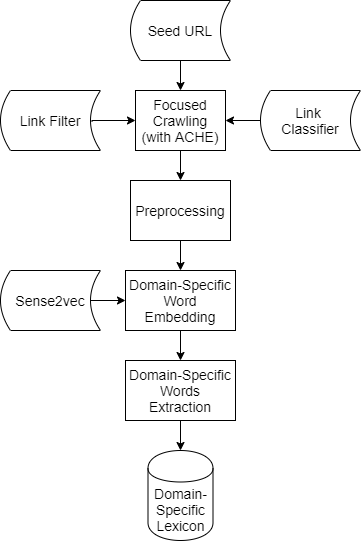
\includegraphics[width=0.3\textwidth]{fig1.png}}
\caption{General architecture of the adapted system.}
\label{fig1}
\end{figure}

\begin{figure}[htbp]
\centerline{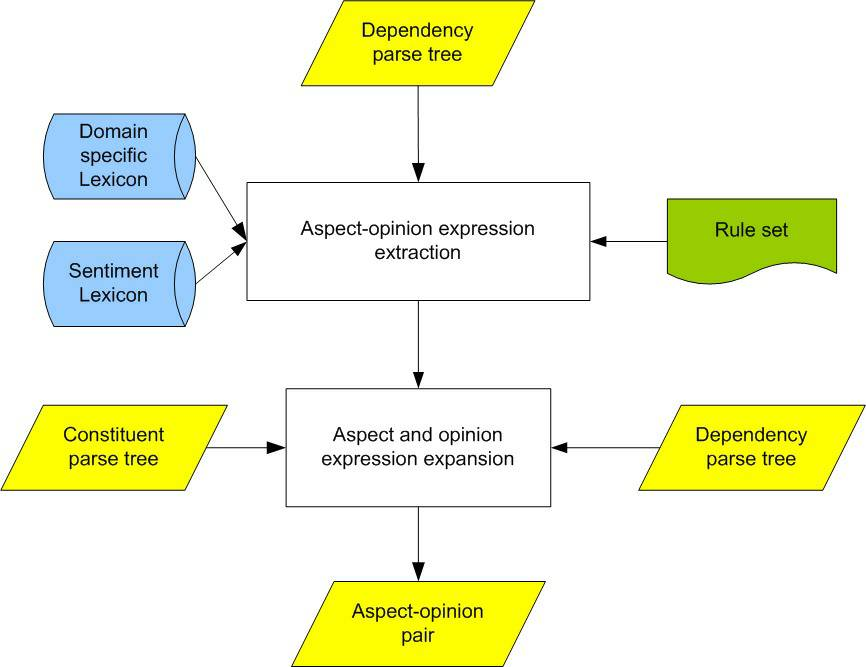
\includegraphics[width=0.45\textwidth]{fig2.jpg}}
\caption{Modified aspect - opinion extraction process.}
\label{fig2}
\end{figure}

To determine the threshold for similarity value used in the extraction process, we experimented with a range of values from 0.1 to 0.9. Then, we conducted the extraction process using these values. Afterwards, we compared the performance of each extraction process and selected the threshold value of 0.3 which gave us the best F1 score.

\section{Development of Domain-Specific Lexicon}
The explanations for each component of the system on Fig. 1 are written on the following sections.

\subsection{Focused Crawling}
The tool used in this step is ACHE, which is an open source focused web crawler. There are three important elements needed to start the crawler:

\subsubsection{Seed URL}
List of URLs that will be visited when the crawler starts. We provided about 10 seeds for each domain.

\subsubsection{Link Classifier}
List of words in regex compatible form, used to determine if a web page is relevant to the domain.

\subsubsection{Link Filter}
List of URLs that can be visited by the crawler (whitelist) and cannot be visited by the crawler (blacklist).

The crawling process took about an hour for each domain, resulting in about 3000 crawled web pages per domain. The crawled data is stored in a DEFLATE file consists of JSON objects. Each JSON object contains the details of a web page.

\subsection{Preprocessing}

We performed four steps of preprocessing, as follows:
\subsubsection{Preprocessing on Crawled Data}
First, we checked the relevance of each JSON object in the crawled data. If the object is relevant to the domain, extract its content.

\subsubsection{Cleaning Crawled Data}
To clean crawled data, we deleted every character that is not in ASCII, name of currencies, and whitespace. After that, we split the data to form a file in which each line contains a sentence.

\subsubsection{Preprocessing on a Sentence}
We preprocessed each sentence using a pretrained model from spaCy\footnote{spaCy: https://github.com/explosion/spaCy} to create a Doc. Doc is a data structure from spaCy which contains a sequence of tokens. The process of building a Doc is illustrated on Fig.~\ref{fig3}. After the Doc was built, we continued with token merging.

\begin{figure}[htbp]
\centerline{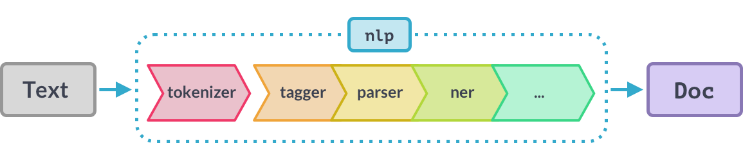
\includegraphics[width=0.47\textwidth]{fig3.png}}
\caption{The process of building a Doc [18].}
\label{fig3}
\end{figure}

\paragraph{Merge Noun Phrase}
In this step, we checked every phrase in the generated noun chunks property from Doc. Noun chunks are phrases which have a noun as the head. If the phrase is prefixed with determiner or conjunction, then the prefix would be removed. If the phrase starts with an adjective or adverb, then it would not be merged, unless it is in the list of exceptions described in Table~\ref{tab1}. 

\begin{table}[htbp]
\caption{List of Exceptions with Examples}
\begin{center}
\begin{tabular}{|c|c|}
\hline
\textbf{Exceptions} & \textbf{Examples}\\
\hline
Phrase is a term in WordNet&digital camera, mineral water\\
\hline
The adjective is a nationality&French, English, Welsh\\
\hline
The adjective is a color&red, blue, yellow\\
\hline
The adjective is an ordinal number&first, second, third\\
\hline
\end{tabular}
\label{tab1}
\end{center}
\end{table}

\paragraph{Merge Named Entities}
The types of named entities that would be merged are name, location, time, number, and money.

\paragraph{Merge Adjective Phrase}
To extract adjective phrase, we used the textacy library which is an extension of spaCy. The extraction is done using the rule described in Fig. 4. The meaning of the pattern is: Find an adjective token, can be followed by an adverb token or not, which is followed by another adjective token and can be followed by another adverb token or not.

\subsubsection{Cleaning a Sentence}
After the preprocessing steps were done, we proceeded to clean each sentence by removing stopwords, URLs, and named entities.

The example of input and final output from the preprocessing steps is displayed on Fig 5. In the output, each token is followed by its part-of-speech (POS) tag obtained from spaCy. While doing the POS tagging, spaCy followed the Universal POS tags format from the Universal Dependencies scheme.

\subsection{Domain-Specific Word Embedding}
To build a domain-specific word embedding, we used an implementation of sense2vec provided by Explosion AI3. The sense2vec model was trained using word2vec via FastText. To avoid using n-gram, we set the value of the maximum n-gram size parameter to 0. There are two types of word2vec model that we used to build the embedding: CBOW and Skip-gram. For each model, we created word vectors of size 300 and 400.

\subsection{Domain-Specific Words Extraction}
At first, we manually labelled every unique word in the preprocessed text into three classes: aspect, opinion, and other (neither an aspect nor an opinion). Then, we used the following approach to choose the words for test data, while the rest of the words were used as the train data:

\subsubsection{Using Term Frequency Only}
In this approach, we used 1000 most frequent words as the test data. Examples of the resulting domain-specific lexicons are shown in Table II.

\subsubsection{Using Term Frequency and Cosine Similarity}
First, we chose 50 most frequent words as the seed words. Next, we expand the seed words using 20 most similar words from each seed. The number of most frequent and most similar words were chosen arbitrarily. Table III shows the resulting domain-specific lexicon.

\subsection{Domain-Specific Word Classification}
After separating train and test data, we classified the words in the test data into their respective classes using supervised and unsupervised approach. The explanations for each approach are as follows:

\subsubsection{Supervised Approach}
\paragraph{SVM Classifier with RBF Kernel}
This classifier was chosen because of its proven ability to produce good results on text classification tasks [15]. For the feature, we used normalized word vectors.

\paragraph{Cosine Similarity}
In this method, we compared the similarity of each word to the averaged word vector of aspect class, averaged word vector of opinion class, and averaged word vector of other class. After that, we chose the nearest averaged word vector as the class.

\subsubsection{Unsupervised Approach}
In this approach, we clustered the word vectors in train data using K-Means and K-Medoids method. Then, we used the computed centroids to predict the test data.

\begin{table*}[htbp]
\caption{List of Exceptions with Examples}
\begin{center}
\begin{tabular}{|c|c|}
\hline
\textbf{Exceptions} & \textbf{Examples}\\
\hline
Phrase is a term in WordNet&digital camera, mineral water\\
\hline
The adjective is a nationality&French, English, Welsh\\
\hline
The adjective is a color&red, blue, yellow\\
\hline
The adjective is an ordinal number&first, second, third\\
\hline
\end{tabular}
\label{tab2}
\end{center}
\end{table*}

\begin{itemize}
\item Use either SI (MKS) or CGS as primary units. (SI units are encouraged.) English units may be used as secondary units (in parentheses). An exception would be the use of English units as identifiers in trade, such as ``3.5-inch disk drive''.
\item Avoid combining SI and CGS units, such as current in amperes and magnetic field in oersteds. This often leads to confusion because equations do not balance dimensionally. If you must use mixed units, clearly state the units for each quantity that you use in an equation.
\item Do not mix complete spellings and abbreviations of units: ``Wb/m\textsuperscript{2}'' or ``webers per square meter'', not ``webers/m\textsuperscript{2}''. Spell out units when they appear in text: ``. . . a few henries'', not ``. . . a few H''.
\item Use a zero before decimal points: ``0.25'', not ``.25''. Use ``cm\textsuperscript{3}'', not ``cc''.)
\end{itemize}

\subsection{Equations}
Number equations consecutively. To make your 
equations more compact, you may use the solidus (~/~), the exp function, or 
appropriate exponents. Italicize Roman symbols for quantities and variables, 
but not Greek symbols. Use a long dash rather than a hyphen for a minus 
sign. Punctuate equations with commas or periods when they are part of a 
sentence, as in:
\begin{equation}
a+b=\gamma\label{eq}
\end{equation}

Be sure that the 
symbols in your equation have been defined before or immediately following 
the equation. Use ``\eqref{eq}'', not ``Eq.~\eqref{eq}'' or ``equation \eqref{eq}'', except at 
the beginning of a sentence: ``Equation \eqref{eq} is . . .''

\subsection{\LaTeX-Specific Advice}

Please use ``soft'' (e.g., \verb|\eqref{Eq}|) cross references instead
of ``hard'' references (e.g., \verb|(1)|). That will make it possible
to combine sections, add equations, or change the order of figures or
citations without having to go through the file line by line.

Please don't use the \verb|{eqnarray}| equation environment. Use
\verb|{align}| or \verb|{IEEEeqnarray}| instead. The \verb|{eqnarray}|
environment leaves unsightly spaces around relation symbols.

Please note that the \verb|{subequations}| environment in {\LaTeX}
will increment the main equation counter even when there are no
equation numbers displayed. If you forget that, you might write an
article in which the equation numbers skip from (17) to (20), causing
the copy editors to wonder if you've discovered a new method of
counting.

{\BibTeX} does not work by magic. It doesn't get the bibliographic
data from thin air but from .bib files. If you use {\BibTeX} to produce a
bibliography you must send the .bib files. 

{\LaTeX} can't read your mind. If you assign the same label to a
subsubsection and a table, you might find that Table I has been cross
referenced as Table IV-B3. 

{\LaTeX} does not have precognitive abilities. If you put a
\verb|\label| command before the command that updates the counter it's
supposed to be using, the label will pick up the last counter to be
cross referenced instead. In particular, a \verb|\label| command
should not go before the caption of a figure or a table.

Do not use \verb|\nonumber| inside the \verb|{array}| environment. It
will not stop equation numbers inside \verb|{array}| (there won't be
any anyway) and it might stop a wanted equation number in the
surrounding equation.

\subsection{Some Common Mistakes}\label{SCM}
\begin{itemize}
\item The word ``data'' is plural, not singular.
\item The subscript for the permeability of vacuum $\mu_{0}$, and other common scientific constants, is zero with subscript formatting, not a lowercase letter ``o''.
\item In American English, commas, semicolons, periods, question and exclamation marks are located within quotation marks only when a complete thought or name is cited, such as a title or full quotation. When quotation marks are used, instead of a bold or italic typeface, to highlight a word or phrase, punctuation should appear outside of the quotation marks. A parenthetical phrase or statement at the end of a sentence is punctuated outside of the closing parenthesis (like this). (A parenthetical sentence is punctuated within the parentheses.)
\item A graph within a graph is an ``inset'', not an ``insert''. The word alternatively is preferred to the word ``alternately'' (unless you really mean something that alternates).
\item Do not use the word ``essentially'' to mean ``approximately'' or ``effectively''.
\item In your paper title, if the words ``that uses'' can accurately replace the word ``using'', capitalize the ``u''; if not, keep using lower-cased.
\item Be aware of the different meanings of the homophones ``affect'' and ``effect'', ``complement'' and ``compliment'', ``discreet'' and ``discrete'', ``principal'' and ``principle''.
\item Do not confuse ``imply'' and ``infer''.
\item The prefix ``non'' is not a word; it should be joined to the word it modifies, usually without a hyphen.
\item There is no period after the ``et'' in the Latin abbreviation ``et al.''.
\item The abbreviation ``i.e.'' means ``that is'', and the abbreviation ``e.g.'' means ``for example''.
\end{itemize}
An excellent style manual for science writers is \cite{b7}.

\subsection{Authors and Affiliations}
\textbf{The class file is designed for, but not limited to, six authors.} A 
minimum of one author is required for all conference articles. Author names 
should be listed starting from left to right and then moving down to the 
next line. This is the author sequence that will be used in future citations 
and by indexing services. Names should not be listed in columns nor group by 
affiliation. Please keep your affiliations as succinct as possible (for 
example, do not differentiate among departments of the same organization).

\subsection{Identify the Headings}
Headings, or heads, are organizational devices that guide the reader through 
your paper. There are two types: component heads and text heads.

Component heads identify the different components of your paper and are not 
topically subordinate to each other. Examples include Acknowledgments and 
References and, for these, the correct style to use is ``Heading 5''. Use 
``figure caption'' for your Figure captions, and ``table head'' for your 
table title. Run-in heads, such as ``Abstract'', will require you to apply a 
style (in this case, italic) in addition to the style provided by the drop 
down menu to differentiate the head from the text.

Text heads organize the topics on a relational, hierarchical basis. For 
example, the paper title is the primary text head because all subsequent 
material relates and elaborates on this one topic. If there are two or more 
sub-topics, the next level head (uppercase Roman numerals) should be used 
and, conversely, if there are not at least two sub-topics, then no subheads 
should be introduced.

\subsection{Figures and Tables}
\paragraph{Positioning Figures and Tables} Place figures and tables at the top and 
bottom of columns. Avoid placing them in the middle of columns. Large 
figures and tables may span across both columns. Figure captions should be 
below the figures; table heads should appear above the tables. Insert 
figures and tables after they are cited in the text. Use the abbreviation 
``Fig.~\ref{fig}'', even at the beginning of a sentence.

\begin{table}[htbp]
\caption{Table Type Styles}
\begin{center}
\begin{tabular}{|c|c|c|c|}
\hline
\textbf{Table}&\multicolumn{3}{|c|}{\textbf{Table Column Head}} \\
\cline{2-4} 
\textbf{Head} & \textbf{\textit{Table column subhead}}& \textbf{\textit{Subhead}}& \textbf{\textit{Subhead}} \\
\hline
copy& More table copy$^{\mathrm{a}}$& &  \\
\hline
\multicolumn{4}{l}{$^{\mathrm{a}}$Sample of a Table footnote.}
\end{tabular}
\label{tab100}
\end{center}
\end{table}


Figure Labels: Use 8 point Times New Roman for Figure labels. Use words 
rather than symbols or abbreviations when writing Figure axis labels to 
avoid confusing the reader. As an example, write the quantity 
``Magnetization'', or ``Magnetization, M'', not just ``M''. If including 
units in the label, present them within parentheses. Do not label axes only 
with units. In the example, write ``Magnetization (A/m)'' or ``Magnetization 
\{A[m(1)]\}'', not just ``A/m''. Do not label axes with a ratio of 
quantities and units. For example, write ``Temperature (K)'', not 
``Temperature/K''.

\section{The Cost and Benefit of Using Domain-Specific Lexicon over Aspect and Opinion List}
To build a domain-specific lexicon, we need labelled data. In our experiments, the labelling process is done manually, making it a rather costly process because it takes time and effort. Some knowledge of the domain is also necessary to make sure that the classes are labelled correctly.

Even so, the scope of the domain-specific lexicon is bigger than the original aspect and opinion list, allowing it to be used for multiple datasets in the same domain. We tried to reduce the cost by using POS tags to roughly split the data into their respective classes before going over the data manually.

\section{Issues on the Domain-Specific Lexicon and Pretrained Word Embedding}
There are multiple issues on the domain-specific lexicon and the pretrained word embedding that could hinder the performance of the modified Sequential Covering method, causing it to not work as effectively as intended. We will address these issues in the following sections.

\subsection{The Extracted Aspect/Opinion Does Not Exist in Word Embedding}
The filtering process in Sequential Covering method uses cosine similarity. If a word does not exist in word embedding (OOV) then the similarity returned would be 0, causing the word to be marked as not relevant to the domain. While building the word embedding, the value of minimum count parameter is set to 5, meaning that if a word appears less than 5 times in the dataset, then it would be regarded as a noise.

An aspect could have a very low frequency because of the change of time causing a difference in aspects that are usually discussed in a review. This is especially more apparent in the product review. Nokia 6610, Canon G3, and Nikon Coolpix 4300 dataset were created in 2004, while the data used to build domain-specific lexicon were crawled in 2020. Example of aspects in the Nokia 6610 dataset that are not in the embeddings: ``CSR", ``PIM", and ``PC Suite".

If an aspect is misspelled in the review dataset, the aspect could also have a very low frequency. For example, the word ``canera" exists as an aspect of the Canon G3 dataset. Because it is a misspelling from the word ``camera", there is a very low chance that the word would exist in the word embedding.

\subsection{No Similar Aspect/Opinion Found in the Domain-Specific Lexicon}
Because of the limitations on the size of domain-specific lexicons that we used in the experiments, some aspect or opinion words may not be included in the domain-specific lexicon. For example, in the Nokia 6610 dataset the aspects: “ring”, “infrared”, “customer service”, “voice dialing”, and “vibration” are not similar with any of the aspects in the domain-specific lexicon for handphone domain.

The smaller the frequency of the aspect/opinion words, the lower the probability that it would be included in the lexicon. To tackle this problem, we suggest to increase the size of domain-specific lexicon or try different combinations of most frequent words and most similar words.

\subsection{Error in Labelled Data Used for Building Domain-Specific Lexicon}
There is a possibility of human error in the data labelling process because it is conducted manually. This problem could cause a decrease in the performance of the modified Sequential Covering method.


\section{Conclusion}
We have adapted the works of Grefenstette and Muchemi [9] to automatically build domain-specific lexicon for the digital camera, handphone, and restaurant domain. In the development of domain-specific lexicon, we obtained the best results for word classification task by using SVM classifier with vectors of size 300 created by CBOW model. The resulting domain-specific lexicons were used in the modified version of Sequential Covering algorithm for aspect extraction [2]. Even though the recalls obtained from the modified method are still lower than the recalls obtained from baseline Sequential Covering, this method managed to yield better F1 scores than the baseline method.

For future works, we suggest increasing the size of the lexicons and using different combinations of most frequent words and most similar words. We also suggest reducing the scope of the domain to create smaller domains such as Nikon digital camera, Canon digital camera, and Nokia phone. By using a smaller domain, we hope that the aspects that are specific to the product would be included in the domain-specific lexicon.


\section*{Acknowledgment}

The preferred spelling of the word ``acknowledgment'' in America is without 
an ``e'' after the ``g''. Avoid the stilted expression ``one of us (R. B. 
G.) thanks $\ldots$''. Instead, try ``R. B. G. thanks$\ldots$''. Put sponsor 
acknowledgments in the unnumbered footnote on the first page.

\section*{References}

Please number citations consecutively within brackets \cite{b1}. The 
sentence punctuation follows the bracket \cite{b2}. Refer simply to the reference 
number, as in \cite{b3}---do not use ``Ref. \cite{b3}'' or ``reference \cite{b3}'' except at 
the beginning of a sentence: ``Reference \cite{b3} was the first $\ldots$''

Number footnotes separately in superscripts. Place the actual footnote at 
the bottom of the column in which it was cited. Do not put footnotes in the 
abstract or reference list. Use letters for table footnotes.

Unless there are six authors or more give all authors' names; do not use 
``et al.''. Papers that have not been published, even if they have been 
submitted for publication, should be cited as ``unpublished'' \cite{b4}. Papers 
that have been accepted for publication should be cited as ``in press'' \cite{b5}. 
Capitalize only the first word in a paper title, except for proper nouns and 
element symbols.

For papers published in translation journals, please give the English 
citation first, followed by the original foreign-language citation \cite{b6}.

\begin{thebibliography}{00}
\bibitem{b1} B. Liu, Sentiment Analysis and Opinion Mining. San Rafael, CA: Morgan and Claypool Publishers, 2012.
\bibitem{b2} F. Z. Ruskanda, D. H. Widyantoro, and A. Purwarianti, ``Sequential covering rule learning for language rule-based aspect extraction," 2019 Int. Conf. on Adv. Comput. Sci. and Inf. Syst. (ICACSIS).
\bibitem{b3} I. S. Jacobs and C. P. Bean, ``Fine particles, thin films and exchange anisotropy,'' in Magnetism, vol. III, G. T. Rado and H. Suhl, Eds. New York: Academic, 1963, pp. 271--350.
\bibitem{b4} K. Elissa, ``Title of paper if known,'' unpublished.
\bibitem{b5} R. Nicole, ``Title of paper with only first word capitalized,'' J. Name Stand. Abbrev., in press.
\bibitem{b6} Y. Yorozu, M. Hirano, K. Oka, and Y. Tagawa, ``Electron spectroscopy studies on magneto-optical media and plastic substrate interface,'' IEEE Transl. J. Magn. Japan, vol. 2, pp. 740--741, August 1987 [Digests 9th Annual Conf. Magnetics Japan, p. 301, 1982].
\bibitem{b7} M. Young, The Technical Writer's Handbook. Mill Valley, CA: University Science, 1989.
\end{thebibliography}
\vspace{12pt}
\color{red}
IEEE conference templates contain guidance text for composing and formatting conference papers. Please ensure that all template text is removed from your conference paper prior to submission to the conference. Failure to remove the template text from your paper may result in your paper not being published.

\end{document}
